\section{Diskusion}
\label{sec:diskusion}
Vi har implementeret en virtuel hukommelse, der har de tre foreslåede sideudskiftningsalgoritmer random, fifo og custom til rådighed. Derudover har vi implementeret en fjerde algoritme, som vi kalder Optimeret random, der laver færre disktilgange end de andre tre.

Der er lavet statestik over hvor ofte disken tilgås, når sideudskiftningsalgoritmerne kører de tre testprogrammer, der alle har vidt forskellige hukommelseadgangs mønstre. 

\subsection{Statistik for sideudskiftningsalgoritmer}
\label{subsec:statistik}
De tre simulerede programkørsler rand, scan og focus er blevet kørt 100 gange med de tre forskellige sideskiftningsalgoritmer. Der er samlet statistik over hvor mange disktilgange de forskellige algoritmer har med et skiftende antal fysiske sider. Programkørslerne resulterede i meget forskellig opførsel i antallet af disk tilgange. I dette afsnit beskrives diskuteres de forskellige resultater, alle kørslerne i en graf kan ses i figur \ref{fig:all}. Vi vil udelukkende forholde os til disktilgange, selvom det også er relevant at se på hvilket overhead en algoritme tilføjer systemet.


\begin{figure}[ht]
\centerline{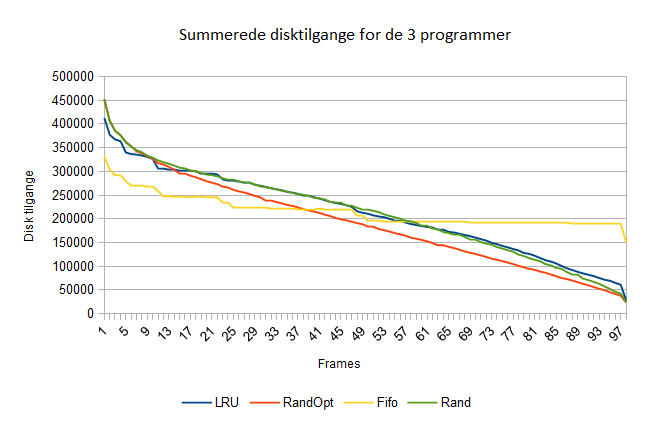
\includegraphics[scale=0.8]{graph/stat_all}}=1]{graph/stat_all}}
\FloatBarrier
\caption{Summeret kørsler for alle programmer med 100 sider}
\label{fig:all}
\end{figure}

\subsubsection{Sekventielle løb}
Programmet "Scan" består af 10 sekventielle løb gennem alt data. Det kan hverken FIFO eller LRU håndtere særlig godt, da begge algoritmer bygger på den antagelse at der er størst sandsynlighed for at data der lige er blevet brugt, snart skal bruges igen. Ved sekventielle gennemløb er det det omvendte der er tilfældet. Dette viste sig også at være tilfældet for FIFO, LRU klarede sig derimod bedre end forventet hvilket skyldes, at LRU implementation ikke nødvendigvis benytter sig af FIFO i tilfælde hvor to sider har end historik (Se. \ref{ssec:custom}).

\begin{figure}[ht]
\centerline{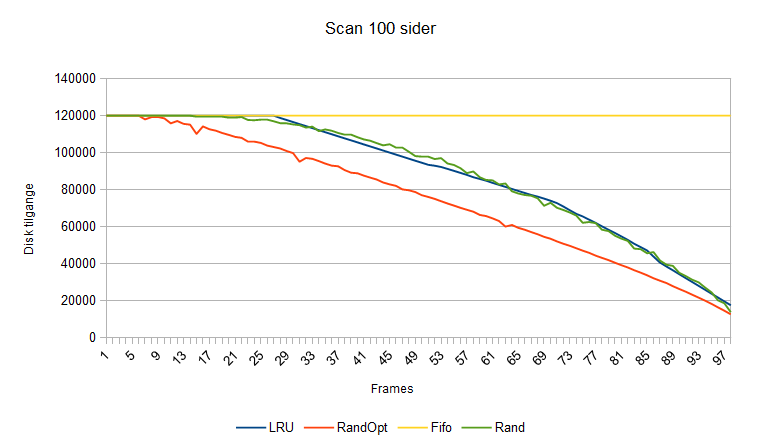
\includegraphics[scale=0.8]{graph/stat_scan}}
\caption{100 Scan kørsler for hvert antal frames summeret}
\label{fig:scan}
\end{figure}

\subsubsection{Anden programkørsel}
Selvom det ikke er unormalt for programmer at have sekventielle gennemløb af data, så er det ikke nødvendigvis normal programkørsel. Programmerne "Focus" og "Sort" har en anden hukkomelses opførsel, der stadigvæk har sekventielle løb, men indenfor mindre dataområder\footnote{Ingen af programmerne har dog et mønster der minder om det der ses i "Operating System Concepts", side 420}. Med disse adgangsmønstre fungerer både FIFO og LRU væsenligt bedre som set i nedenstående figurer. Dog virker de to algoritmer der basere sig på tilfældighed stadigvæk bedre når 50\%+ af siderne er dækket af frames. 

\begin{figure}[ht]
\centerline{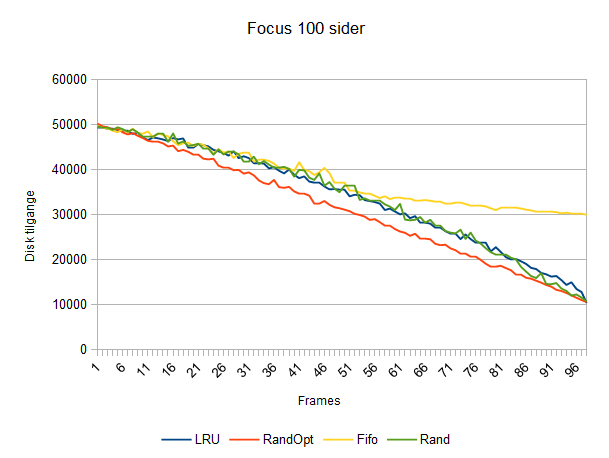
\includegraphics[scale=0.8]{graph/stat_focus}}
\caption{100 focus kørsler for hvert antal frames summeret}
\label{fig:focus}
\end{figure}

\begin{figure}[ht]
\centerline{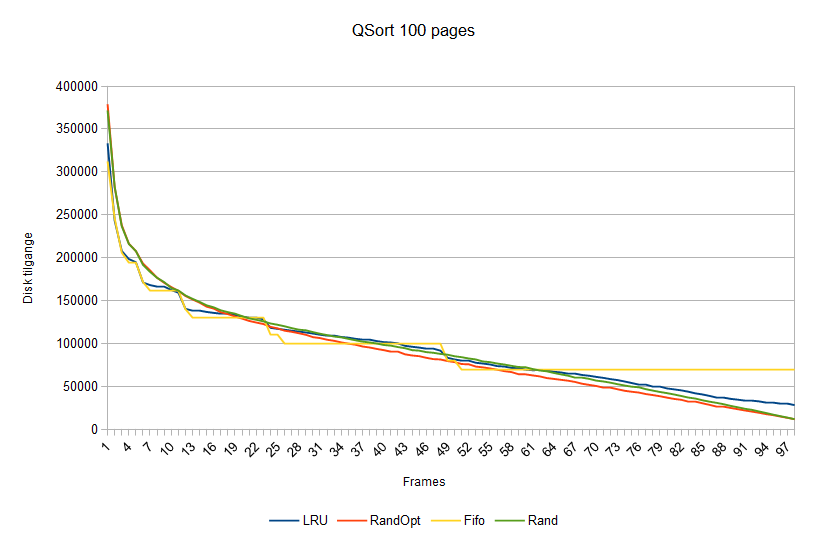
\includegraphics[scale=0.8]{graph/stat_sort}}
\caption{100 sort kørsler for hvert antal frames summeret}
\label{fig:sort}
\end{figure}

\subsection{Konklusion}
Umiddelbart lader det til at algoritmerne der er baseret på tilfældighed resulterer i færre disk tilgange. Der er dog to forbehold, som gør resultatet usikkert. For det første ser det ud til at FIFO og LRU klare sig godt når der er få frames i forhold til sider, for det andet mener vi at en algoritme som OptRand kan få problemer ved lange programkørsler, fordi at der vil end med at være få frames med læserettigheder som der bliver kæmpet om. Det vil givetvis føre til et øget andet antal sideudskiftninger, som vi måske ikke har observeret. Grundlæggende må vi konkludere, at det er de konkrete programkørsler der er bestemmende for, hvornår en given algoritme er god eller dårlig. 
